\chapter{Temperature from Entropy and Energy}

\lectureoverview{Temperature first appears as a conversion of human
thermometer units into microscopic energy units. After making the
corresponding conversion from thermodynamic entropy to dimensionless
statistical entropy, we describe equilibrium by a one-parameter family of
probability distributions. The derivative \(dE/dS\) then defines temperature,
and the first two laws show why a temperature difference determines the
direction of energy flow.}

\section{Conversion Factors and Human Units}

Many constants of physics are conversion factors. The speed of light converts
a distance into a time:
\begin{equation}
 t=\frac{x}{c}.
\end{equation}
If distances and times are measured in compatible units, one may set \(c=1\).
No physical effect disappears; the two kinds of measurement have simply been
put on one common scale.

Boltzmann's constant has the same character. It converts the temperature read
on a human-scale thermometer into an energy. The adjective
\emph{human-scale} is important. Such units are chosen because macroscopic
instruments can produce and resolve them, not because microscopic dynamics
singles them out.

The Celsius degree was fixed by dividing the interval between the freezing and
boiling points of water at standard pressure into one hundred parts. Kelvin
uses a degree of the same size but places zero at absolute zero. Choosing a
different substance, a different interval, or Fahrenheit degrees would change
the numbers but not the physics.

\begin{classroomqa}
\audiencequestion{Was Fahrenheit's scale already a seventeenth-century
construction?}
\lecturerresponse{The precise date is not needed here. The point is that all
such scales were designed around temperatures that people could prepare and
measure. Their degree size is conventional rather than microscopic.
\lecturetimestamp{00:01:34--00:01:50}}
\end{classroomqa}

At the time these scales were created, the molecular origin of heat was not
available to experiment. A one-degree change could be observed with a
macroscopic thermometer, whereas the energy of one molecule could not be
measured. It was therefore natural to invent a temperature unit before anyone
knew that temperature is fundamentally an energy scale.

\section{Why Temperature Has Units of Energy}

Consider a dilute monatomic gas. Dilute means that interaction energies between
molecules may be neglected for the present purpose. In thermal equilibrium,
equipartition assigns \(T_{\mathrm K}/2\) times Boltzmann's constant to each
quadratic translational degree of freedom. In three spatial dimensions,
\begin{equation}
 \left\langle E_{\mathrm{kin}}\right\rangle
 =\frac{3}{2}k_{\mathrm B}T_{\mathrm K}.
 \label{eq:sm2-equipartition-kelvin}
\end{equation}
The factor three counts motion in the \(x\), \(y\), and \(z\) directions. The
factor one-half comes from the quadratic kinetic energy.

This relation is not peculiar to one molecular species. In a mixture of helium
and oxygen at equilibrium, every freely translating particle has the same
average center-of-mass kinetic energy, even though the heavier particles move
more slowly. Since
\begin{equation}
 E_{\mathrm{kin}}=\frac{1}{2}mv^2,
\end{equation}
equal characteristic energy implies \(v\propto m^{-1/2}\).

The same idea can be pushed to a deliberately extreme example. Suspend a
bowling ball in a fluid and let the complete system reach equilibrium. Its
Brownian translational degrees of freedom are governed by the same energy
scale as those of a molecule. The ball's velocity is fantastically smaller
because its mass is fantastically larger, but temperature compares energy
scales, not speeds.

At room temperature, \(T_{\mathrm K}\) is about \(300\,\mathrm K\), while the
energy of one microscopic degree of freedom is tiny in joules. Consequently
the conversion factor is tiny:
\begin{equation}
 k_{\mathrm B}\simeq 1.38\times10^{-23}\,
 \mathrm{J\,K^{-1}}.
 \label{eq:sm2-boltzmann-value}
\end{equation}
Its scale and Avogadro's number are related rather than coincidental:
\begin{equation}
 R=N_{\mathrm A}k_{\mathrm B}.
\end{equation}
The gas constant \(R\) describes a mole, whereas \(k_{\mathrm B}\) describes
the corresponding scale per microscopic constituent.

Fundamental formulas repeatedly contain the combination
\(k_{\mathrm B}T_{\mathrm K}\). It is therefore cleaner to define
\begin{equation}
 T\equiv k_{\mathrm B}T_{\mathrm K}.
 \label{eq:sm2-energy-temperature}
\end{equation}
From now on \(T\) itself has units of energy, and
\eqref{eq:sm2-equipartition-kelvin} becomes
\begin{equation}
 \left\langle E_{\mathrm{kin}}\right\rangle=\frac{3}{2}T.
 \label{eq:sm2-equipartition-natural}
\end{equation}
If energy is measured in joules, temperature is measured in joules. If energy
is measured in electron volts, temperature is measured in electron volts.
There is no new unit of nature called a temperature unit.

\section{Two Conventions for Entropy}

The same conversion appears on the entropy side. Macroscopic thermodynamics
grew out of the analysis of heat engines. Carnot supplied the decisive engine
reasoning; Clausius later introduced the thermodynamic entropy and the symbol
\(S\). In the notation used here, call that macroscopic quantity
\(S_{\mathrm C}\). Its units are energy divided by thermometer temperature,
for example joules per kelvin.

Statistical entropy is dimensionless. For a discrete distribution,
\begin{equation}
 S=-\sum_i p_i\log p_i.
 \label{eq:sm2-statistical-entropy}
\end{equation}
With natural logarithms a fair binary alternative has entropy \(\log2\); with
base-two logarithms the same amount is called one bit. The two entropy
conventions are related by
\begin{equation}
 S=\frac{S_{\mathrm C}}{k_{\mathrm B}},
 \qquad
 S_{\mathrm C}=k_{\mathrm B}S.
 \label{eq:sm2-entropy-conversion}
\end{equation}
A macroscopic value modest in \(\mathrm{J\,K^{-1}}\) corresponds to an
enormous dimensionless entropy because it counts information distributed
among an enormous number of microscopic constituents.

Equations \eqref{eq:sm2-energy-temperature} and
\eqref{eq:sm2-entropy-conversion} establish the convention used throughout:
\[
 [T]=[\text{energy}],
 \qquad
 [S]=1.
\]
Boltzmann's constant may now disappear from the working formulas. It can
always be restored by replacing \(T\) with \(k_{\mathrm B}T_{\mathrm K}\) and
\(S\) with \(S_{\mathrm C}/k_{\mathrm B}\).

\begin{classroomqa}
\audiencequestion{Apart from the factor \(3/2\), is the new temperature simply
an energy measured in joules?}
\lecturerresponse{Yes, if joules are the chosen energy unit. A joule is the
MKS unit \(\mathrm{kg\,m^2\,s^{-2}}\). One could instead use electron volts or
any other energy unit; temperature must then be expressed in that same unit.
The factor \(3/2\) belongs to the ideal-gas example, not to the definition of
temperature.
\lecturetimestamp{00:15:49--00:16:45}}
\end{classroomqa}

\begin{classroomqa}
\audiencequestion{If the board specifies kelvin, is \(k_{\mathrm B}\) not then
a definite constant?}
\lecturerresponse{It is definite after both the temperature and energy units
have been specified. Change kelvin to Fahrenheit degrees, or joules to
electron volts, and its numerical value changes. That unit dependence is
exactly the behavior of a conversion factor.
\lecturetimestamp{00:16:46--00:18:33}}
\end{classroomqa}

\begin{classroomqa}
\audiencequestion{Is the numerical value of Boltzmann's constant determined
experimentally?}
\lecturerresponse{Yes. Historically its evaluation required microscopic
information about atoms and their number density. Boltzmann understood the
relation between molecular energy and temperature before those quantities
were known precisely, much as Newton knew the role of the gravitational
constant before it had been measured accurately.
\lecturetimestamp{00:18:46--00:20:00}}
\end{classroomqa}

\section{Equilibrium Is a Statistical State}

The unit conversion still has not defined temperature. Touching something hot
gives a useful biological intuition, but temperature is a derived physical
quantity built from energy and entropy.

Imagine a system in contact with a large environment whose macroscopic
conditions are fixed. Energy can pass between them. If the system initially
has too much energy, it loses energy on average; if it has too little, it gains
energy on average. In thermal equilibrium microscopic exchanges continue, but
there is no net average flow in either direction.

Let \(i\) label an exact microscopic state of the system and let \(E_i\) be
that state's energy. Equilibrium does not mean that the system freezes in one
state. Its interaction with the environment continually changes the
microstate, so we assign a probability \(P_i\) to each possibility. The basic
relations are
\begin{align}
 \sum_i P_i &=1,
 \label{eq:sm2-normalization}\\
 \sum_i P_iE_i &=\overline E,
 \label{eq:sm2-mean-energy}\\
 S&=-\sum_iP_i\log P_i.
 \label{eq:sm2-equilibrium-entropy}
\end{align}
The bar on \(\overline E\) emphasizes that the subsystem's energy fluctuates.
One measurement may give one value and the next another; repeated
measurements settle into the distribution whose mean is
\eqref{eq:sm2-mean-energy}.

\begin{figure}[t]
\centering

\includegraphics[width=0.82\textwidth]{lecture_02_figure_02.png}
\caption{Normalization and average energy on the board:
\(\sum_iP(i)=1\) and \(\sum_iP(i)E(i)=\langle E\rangle\).}
\lectureframe{00:24:10}
\end{figure}

\section{A Family Labeled by Mean Energy}

The equilibrium distribution depends strongly on the mean energy. Put a pot
of water on a stove and \(\overline E\) rises; put it in the snow and
\(\overline E\) falls. The probabilities change with it. Equilibrium should
therefore be regarded not as one distribution but as a one-parameter family:
\begin{equation}
 P_i(\overline E).
 \label{eq:sm2-family}
\end{equation}
Every member satisfies
\begin{align}
 \sum_iP_i(\overline E)&=1,
 \label{eq:sm2-family-normalization}\\
 \sum_iP_i(\overline E)E_i&=\overline E.
 \label{eq:sm2-family-mean}
\end{align}

\begin{figure}[t]
\centering

\includegraphics[width=0.88\textwidth]{lecture_02_figure_03.png}
\caption{The transition to \(P(i,\overline E)\). The earlier normalization,
mean-energy, and entropy equations remain visible while the family of
distributions is introduced.}
\lectureframe{00:26:29}
\end{figure}

For a schematic plot, order the states by increasing \(E_i\). The horizontal
axis may then be read either as the index \(i\) or as the corresponding energy.
Higher mean energy shifts probability weight toward states farther to the
right. Every curve must retain unit total area.

\begin{figure}[t]
\centering

\includegraphics[width=0.88\textwidth]{lecture_02_figure_04.png}
\caption{Several schematic distributions \(P(i,\overline E)\). Curves weighted
farther toward the right have larger mean energy, while each remains
normalized.}
\lectureframe{00:28:40}
\end{figure}

\begin{figure}[t]
\centering
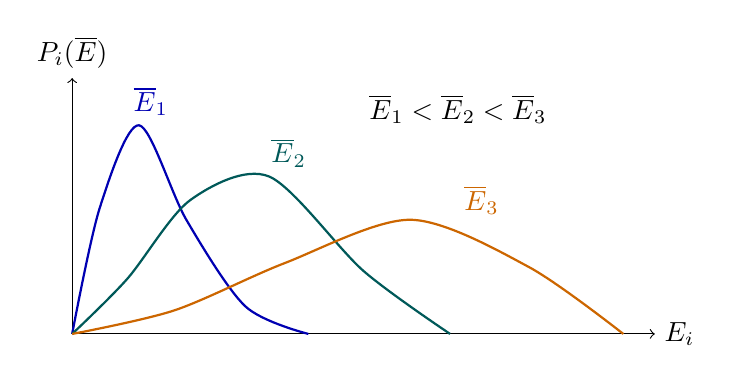
\begin{tikzpicture}[x=1cm,y=1cm]
\draw[->] (0,0) -- (7.4,0) node[right] {$E_i$};
\draw[->] (0,0) -- (0,3.25) node[above] {$P_i(\overline E)$};
\draw[thick,blue!70!black]
  plot[smooth] coordinates {(0,0) (0.35,1.6) (0.85,2.65) (1.45,1.45)
  (2.2,0.35) (3.0,0)};
\draw[thick,teal!70!black]
  plot[smooth] coordinates {(0,0) (0.7,0.7) (1.5,1.7) (2.5,2.0)
  (3.7,0.8) (4.8,0)};
\draw[thick,orange!80!black]
  plot[smooth] coordinates {(0,0) (1.3,0.3) (2.7,0.9) (4.3,1.45)
  (5.8,0.85) (7.0,0)};
\node[blue!70!black] at (1.0,2.95) {\(\overline E_1\)};
\node[teal!70!black] at (2.75,2.3) {\(\overline E_2\)};
\node[orange!80!black] at (5.2,1.7) {\(\overline E_3\)};
\node at (4.9,2.85) {\(\overline E_1<\overline E_2<\overline E_3\)};
\end{tikzpicture}
\caption{A clean version of the board sketch. The curves need not have these
precise shapes; only normalization and their ordered mean energies are being
used.}
\end{figure}

\begin{classroomqa}
\audiencequestion{Is the notation circular? The mean energy is computed from
the distribution, while the distribution is labeled by the mean energy.}
\lecturerresponse{Begin with an empirically selected one-parameter family of
equilibrium distributions. Each member has a mean energy. If distinct members
have distinct means, that mean may be used as the parameter naming the family.
The notation does not yet derive the family; the Boltzmann distribution will
provide that derivation later.
\lecturetimestamp{00:28:35--00:29:44}}
\end{classroomqa}

\begin{classroomqa}
\audiencequestion{Why say average energy rather than total energy?}
\lecturerresponse{The subsystem is exchanging energy with a heat bath, such as
the atmosphere around a gas container with thermally permeable walls. Its
instantaneous energy fluctuates. Many measurements produce a distribution, and
\(\overline E\) is the mean of those outcomes. The energy of the larger closed
system consisting of subsystem plus bath may still be fixed.
\lecturetimestamp{00:29:46--00:30:56}}
\end{classroomqa}

\begin{classroomqa}
\audiencequestion{Can different microscopic states have the same energy, and
can different distributions have the same mean energy?}
\lecturerresponse{Both are possible. The mean-energy constraint by itself
allows many distributions, so the special one-parameter equilibrium family
requires an additional physical argument. Its origin and its Boltzmann form
will be derived later. Equal energies of distinct microstates are the separate
issue called degeneracy.
\lecturetimestamp{00:30:58--00:32:22}}
\end{classroomqa}

\subsection{State labels, degeneracy, and correlation}

Several distinctions that are easy to blur must be kept separate.

First, many probability distributions can have the same mean energy. The
one-parameter equilibrium family is not obtained from the mean-energy
constraint alone. It is the particular family selected by equilibration; its
form will later be identified as the Boltzmann distribution.

Second, several different microstates can have the same energy. This is called
degeneracy. The board discussion temporarily ignores exact degeneracies so
that the states can be ordered unambiguously by energy. Degeneracy is in fact
common when a system has symmetries, but it causes no conceptual problem:
retain the state label \(i\), allow repeated values of \(E_i\), and sum over
all states.

Third, correlation is not another word for degeneracy. Correlation concerns a
joint distribution of two random quantities and asks whether knowing one
changes the probabilities for the other. The mutually exclusive labels
\(i\) and \(j\) in one list of microstates are not, by themselves, two random
variables whose correlation is being computed.

\begin{classroomqa}
\audiencequestion{Does the construction assume that different \(i\)-states
are independent, and what if two of them are correlated?}
\lecturerresponse{A state label is one possible value of a single microscopic
random variable. Independence and correlation require two jointly distributed
variables, so that terminology does not apply directly to two alternative
labels in this list. Equal energies of distinct states are instead a question
about degeneracy.
\lecturetimestamp{00:32:23--00:33:22}}
\end{classroomqa}

\begin{classroomqa}
\audiencequestion{What if two distinct states have exactly the same energy?}
\lecturerresponse{That is degeneracy. For the immediate graph we adopt the
simplifying assumption that no two energies coincide and order the states by
increasing energy. The later probability formulas do not require this
assumption; degenerate states are simply counted separately.
\lecturetimestamp{00:33:23--00:34:04}}
\end{classroomqa}

\begin{classroomqa}
\audiencequestion{Is the meaning of the index \(i\) arbitrary?}
\lecturerresponse{The microscopic states themselves are not arbitrary: each
specifies all positions, momenta, or other data needed for an exact
description. Their names are arbitrary, so for the picture we choose labels in
ascending order of energy.
\lecturetimestamp{00:34:06--00:35:15}}
\end{classroomqa}

\section{Entropy Becomes a Function of Energy}

Every member of the equilibrium family has an entropy. Substituting
\eqref{eq:sm2-family} into \eqref{eq:sm2-equilibrium-entropy} gives
\begin{equation}
 S(\overline E)
 =-\sum_iP_i(\overline E)\log P_i(\overline E).
 \label{eq:sm2-entropy-energy}
\end{equation}
This is not one universal function shared by all physical systems. It depends
on the system's spectrum and on its equilibrium family. Once that family is
specified, however, energy and entropy are linked: moving through the family
changes both.

Ordinary systems typically spread their probability over more states as their
mean energy rises, so \(S\) usually rises with \(\overline E\). For now we
assume that this relation is smooth and locally invertible. The exceptions are
important, but the simple case exposes the definition we need.

\section{The Derivative That Defines Temperature}

Ask a concrete question: how much must the mean energy change in order to
increase the entropy by one binary alternative? In natural-log units that
entropy increment is \(\log2\).

For neighboring members of a smooth family,
\begin{equation}
 dE=\frac{dE}{dS}\,dS.
 \label{eq:sm2-differential-identity}
\end{equation}
At this point the equation is only the chain rule. Its coefficient, however,
has exactly the dimensions and physical role required of temperature.

\begin{definition}
The temperature in energy units is
\begin{equation}
 T\equiv\frac{dE}{dS}.
 \label{eq:sm2-temperature-definition}
\end{equation}
Equivalently,
\begin{equation}
 dE=T\,dS,
 \qquad
 dS=\frac{1}{T}\,dE.
 \label{eq:sm2-fundamental-differentials}
\end{equation}
\end{definition}

For a sufficiently small change of one bit,
\begin{equation}
 \Delta E\simeq T\log2.
 \label{eq:sm2-one-bit-energy}
\end{equation}
The fixation on one bit is only a way to make the derivative tangible. Any
small entropy change obeys the same local relation.

\begin{classroomqa}
\audiencequestion{Since entropy was written as \(S(E)\), would
\(dS/dE\) not be the more natural derivative?}
\lecturerresponse{Either derivative contains the same information when the
relation is locally invertible:
\[
 \frac{dE}{dS}=\left(\frac{dS}{dE}\right)^{-1}.
\]
Temperature is conventionally \(dE/dS\), while inverse temperature is
\(dS/dE=1/T\).
\lecturetimestamp{00:40:24--00:40:54}}
\end{classroomqa}

Only one thermodynamic variable is changing here, so ordinary derivatives are
sufficient. When volume, particle number, magnetization, or other variables
are allowed to change, one must use partial derivatives and state which
quantities are held fixed. The present definition is the one-variable slice
of that more general thermodynamic geometry.

\subsection{Why Boltzmann's constant cancels}

Return briefly to thermometer units. Using
\[
 T=k_{\mathrm B}T_{\mathrm K},
 \qquad
 S=\frac{S_{\mathrm C}}{k_{\mathrm B}},
\]
the fundamental relation becomes
\begin{align}
 dE
 &=\bigl(k_{\mathrm B}T_{\mathrm K}\bigr)
   d\left(\frac{S_{\mathrm C}}{k_{\mathrm B}}\right)\\
 &=T_{\mathrm K}\,dS_{\mathrm C}.
 \label{eq:sm2-carnot-form}
\end{align}
One factor of \(k_{\mathrm B}\) enters through temperature and the reciprocal
factor enters through entropy. They cancel. This is why a conventional
thermodynamics text can write \eqref{eq:sm2-carnot-form} without displaying
Boltzmann's constant.

\begin{classroomqa}
\audiencequestion{Must \(S(E)\) be invertible?}
\lecturerresponse{Not always. For ordinary systems in the regime considered
here, increasing energy generally broadens the equilibrium distribution and
increases entropy, so \(S(E)\) is monotone and \(T>0\). Systems with bounded
spectra can provide counterexamples, including regimes in which entropy
decreases with energy and the statistical temperature is negative. We set
those cases aside for now.
\lecturetimestamp{00:44:30--00:45:57}}
\end{classroomqa}

\section{From the Abstract Derivative to Hot and Cold}

The derivative definition is universal but still abstract. We want to recover
the familiar statement that energy flows from a hotter body to a colder one.
Pain from touching a hot surface is biological; color and emitted radiation
depend on the properties of light. A statistical definition should also make
sense for an idealized gas even when radiation is ignored.

\begin{classroomqa}
\audiencequestion{Could the light emitted by a hot object provide the basic
definition of temperature?}
\lecturerresponse{Radiation is a useful thermometer, but it introduces the
physics of light. Statistical mechanics must define temperature for systems
such as a box of gas without relying on optical properties. The direction of
energy exchange is the more general criterion.
\lecturetimestamp{00:46:42--00:47:20}}
\end{classroomqa}

Prepare two systems \(A\) and \(B\), each initially in its own equilibrium,
with temperatures \(T_A\) and \(T_B\). They are initially isolated from one
another. Then connect them through a weak thermal contact: the
\emph{thin pipe} allows small amounts of energy to pass back and forth without
destroying the identity of either subsystem.

\begin{figure}[t]
\centering

\includegraphics[width=0.88\textwidth]{lecture_02_figure_05.png}
\caption{The separately prepared systems \(A\) and \(B\), labeled by
temperatures \(T_A\) and \(T_B\), just before weak thermal contact is
considered.}
\lectureframe{00:48:55}
\end{figure}

\begin{figure}[t]
\centering
\begin{tikzpicture}[>=Stealth]
\draw[rounded corners,thick,fill=blue!6] (0,0) rectangle (2.6,2.4);
\draw[rounded corners,thick,fill=orange!8] (5.4,0) rectangle (8,2.4);
\draw[thick] (2.6,1.35) -- (5.4,1.35);
\draw[thick] (2.6,1.05) -- (5.4,1.05);
\draw[<->,very thick] (3.15,1.2) -- (4.85,1.2)
  node[midway,above] {\(\delta E\)};
\node at (1.3,1.45) {\Large \(A\)};
\node at (6.7,1.45) {\Large \(B\)};
\node at (1.3,0.65) {\(T_A,S_A,E_A\)};
\node at (6.7,0.65) {\(T_B,S_B,E_B\)};
\node at (4,0.35) {\small weak thermal contact};
\end{tikzpicture}
\caption{Energy fluctuates through the weak contact while the combined system
remains isolated.}
\end{figure}

Suppose, without loss of generality,
\begin{equation}
 T_B>T_A.
 \label{eq:sm2-temperature-order}
\end{equation}
Experience says that \(B\) should lose energy and \(A\) should gain it. Three
facts turn that expectation into a calculation.

\subsection{Entropy additivity}

For two weakly coupled subsystems whose microscopic alternatives combine
independently, the number of joint possibilities multiplies:
\[
 W_{AB}=W_AW_B.
\]
Entropy is logarithmic, so
\begin{equation}
 S_{\mathrm{tot}}=S_A+S_B.
 \label{eq:sm2-entropy-additivity}
\end{equation}
The same result follows directly from the Shannon entropy of a product
distribution.

\begin{classroomqa}
\classquestion{Why does the entropy of the combined system add?}
\lecturerresponse{Because the underlying number of alternatives multiplies
while entropy takes a logarithm:
\(\log(W_AW_B)=\log W_A+\log W_B\). Weak interaction is what permits the
subsystem description and this leading additive form.
\lecturetimestamp{00:51:06--00:52:03}}
\end{classroomqa}

\subsection{The first and second laws}

The combined system is isolated, so energy exchanged internally is conserved:
\begin{equation}
 dE_A+dE_B=0,
 \qquad
 dE_B=-dE_A.
 \label{eq:sm2-first-law}
\end{equation}
This is the first law in the present experiment.

The second law is taken here as a postulate to be explained more deeply later.
As the connected systems relax toward their new equilibrium,
\begin{equation}
 dS_{\mathrm{tot}}=dS_A+dS_B\geq0.
 \label{eq:sm2-second-law}
\end{equation}
The strict inequality describes spontaneous relaxation away from equilibrium;
equality holds at equilibrium for the reversible first-order variation.

Finally, the temperature definition applies to each subsystem:
\begin{equation}
 dE_A=T_A\,dS_A,
 \qquad
 dE_B=T_B\,dS_B.
 \label{eq:sm2-two-temperatures}
\end{equation}

\begin{figure}[H]
\centering

\includegraphics[width=0.88\textwidth]{lecture_02_figure_06.png}
\caption{The two subsystem relations
\(dE_A=T_A\,dS_A\) and \(dE_B=T_B\,dS_B\) at the close of the board
argument.}
\lectureframe{00:54:00}
\end{figure}

\subsection{The sign of the energy flow}

These equations already fix the direction of net transfer. Substitute
\(dS_A=dE_A/T_A\), \(dS_B=dE_B/T_B\), and
\eqref{eq:sm2-first-law} into \eqref{eq:sm2-second-law}:
\begin{align}
 dS_{\mathrm{tot}}
 &=\frac{dE_A}{T_A}+\frac{dE_B}{T_B}\\
 &=dE_A\left(\frac{1}{T_A}-\frac{1}{T_B}\right)\geq0.
 \label{eq:sm2-flow-sign}
\end{align}
If \(T_B>T_A>0\), then
\[
 \frac{1}{T_A}-\frac{1}{T_B}>0.
\]
Equation \eqref{eq:sm2-flow-sign} therefore requires
\[
 dE_A>0,
 \qquad
 dE_B<0.
\]
The colder system \(A\) gains energy and the hotter system \(B\) loses it.
When \(T_A=T_B\), the first-order entropy change supplies no preferred
direction, and microscopic exchanges balance to zero net flow. Thus the
abstract derivative \(T=dE/dS\) reproduces the operational distinction between
hot and cold.
